\chapter{\babEmpat}
\label{bab:4}

Bab ini membahas mengenai proses \f{fine tuning} model \f{Bidirectional Encoder Representations from Transformers} (BERT) untuk mendapatkan model yang dapat digunakan pada masalah pemeringkatan teks.
\sect~\ref{sec:spesifikasi} menjelaskan mengenai spesifikasi perangkat keras dan perangkat lunak yang digunakan dalam penelitian. Selanjutnya, \sect~\ref{sec:simulasi} menjelaskan mengenai tahapan simulasi yang dilakukan dalam penelitian. Informasi mengenai \f{dataset} latih dan uji  dijelaskan pada \sect~\ref{sec:dataset}. \sect~\ref{sec:finetuning} menjelaskan lebih detail mengenai arsitektur model BERT, fungsi loss, serta konfigurasi \f{hyperparameter} yang digunakan dalam proses \f{fine tuning} model BERT. Terakhir, \sect~\ref{sec:hasil} menjelaskan mengenai evaluasi hasil \f{fine tuning} model BERT untuk pemeringkatan teks.

\section{Spesifikasi Mesin dan Perangkat Lunak}
\label{sec:spesifikasi}

Proses \f{fine tuning} model BERT untuk pemeringkatan teks dilakukan menggunakan mesin dan perangkat lunak yang tertera pada \tab~\ref{tab:spesifikasi}.
\begin{table}[!ht]
    \centering
    \caption{Spesifikasi perangkat lunak yang digunakan pada penelitian ini.}
    \label{tab:spesifikasi}
    \begin{tabular}{|l|l|} \hline
        \textbf{CPU}                         & AMD Ryzen 9 5950X 32-Core Processor                                                                                                      \\ \hline
        \textbf{GPU}                         & NVIDIA GeForce RTX 4090 24GB                                                                                                             \\ \hline
        \textbf{Memori}                      & 64GB                                                                                                                                     \\ \hline
        \textbf{Sistem Operasi}              & Ubuntu 20.04.2 LTS                                                                                                                       \\ \hline
        \textbf{Perangkat Lunak Pemrograman} & Visual Studio Code 1.84.2                                                                                                                \\ \hline
        \textbf{Bahasa Pemrograman}          & Python 3.8                                                                                                                               \\ \hline
        \textbf{Pustaka yang Digunakan}      & \begin{tabular}[c]{@{}l@{}}sentence-transformers 2.2.2\\ transformers 4.35.1\\ beir 2.0.0\\ gdown 4.7.1\\ torch 2.0.1+cu117\end{tabular} \\ \hline
    \end{tabular}
\end{table}

\section{Tahapan Simulasi}
\label{sec:simulasi}

\pic~\ref{fig:diagram-simulasi} menunjukkan tahapan simulasi yang dilakukan dalam penelitian ini.
\begin{figure}[!ht]
    \centering
    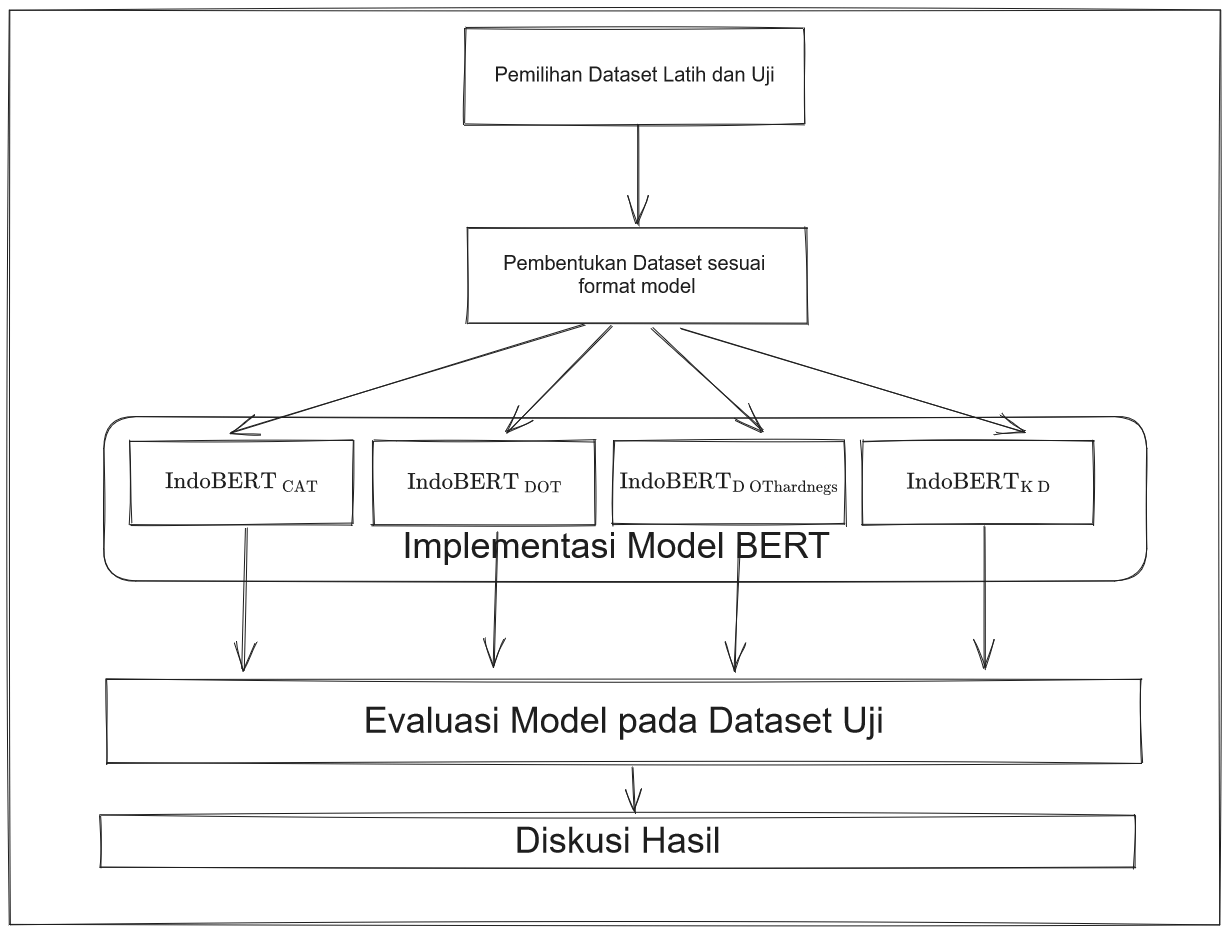
\includegraphics[width=1\textwidth]{assets/pics/alursimulasi.png}
    \caption{Diagram Simulasi}
    \label{fig:diagram-simulasi}

\end{figure}

Simulasi diawali dengan pengambilan data. Data yang digunakan adalah data pada penelitian \cite{mmarco}, sebagai \f{dataset} latih, dan data pada penelitian \cite{mrtydi}, \cite{miracl} sebagai \f{dataset} uji. \f{Dataset} latih tidak dapat digunakan langsung untuk melatih model-model tersebut. Untuk setiap modelnya, diperlukan transformasi untuk mengubah bentuk dari \f{dataset} latih sehingga sesuai dengan formatnya. Transformasi \f{dataset} latih dan \f{hyperparameter} dari model akan dibahas lebih lanjut pada bagian \sect~\ref{sec:finetuning}. Selanjutnya, proses implementasi dan pelatihan model dilakukan. Setelah itu, akan dilakukan evaluasi setiap model pada \f{dataset} uji. Terdapat satu model BM25 sebagai \f{baseline} untuk membandingkan hasil evaluasi dari model-model yang dilatih. Terakhir, terdapat diskusi mengenai hasil evaluasi untuk setiap model.

\section{Data}
\label{sec:dataset}

Penelitian ini menggunakan satu \f{dataset} latih mMarco \f{train set} bahasa Indonesia \citep{mmarco} dan tiga \f{dataset} uji, yaitu mMarco \f{dev set} bahasa Indonesia, MrTyDi Test set Indonesia \citep{mrtydi}, dan Miracl \f{dev set} bahasa Indonesia \citep{miracl}. \f{Dataset} Miracl dan MrTyDi dipilih sebagai uji kemampuan \f{out-of-distibution} dari model yang dihasilkan. Setiap \f{dataset} terdiri dari 3 \f{file}, yaitu \f{file} kueri, \f{file} korpus dan \f{file jugdements} yang telah dijelaskan pada \sect~\ref{sec:dataset-umum}. \tab~\ref{tab:dataset-info} menunjukkan informasi mengenai jumlah entri dari \f{file} kueri, \f{file} korpus, dan \f{file jugdements} dari setiap \f{dataset} yang digunakan dalam penelitian ini.
\begin{table}[!ht]
    \centering
    \caption{Tabel Informasi untuk Setiap \f{Dataset}. Kolom \f{Korpus} menunjukkan jumlah entri pada \f{file korpus}, kolom \f{Kueri} menunjukkan jumlah entri pada \f{file kueri}, dan kolom \f{Jugdements} menunjukkan jumlah entri pada \f{file jugdements} (pasangan kueri dan teks dengan nilai relevansi).}
    \label{tab:dataset-info}
    \begin{tabular}{|l|c|c|r| r|} \hline
        \textbf{Dataset} & \textbf{Korpus} & \textbf{Kueri} & \textbf{Jugdements} & \textbf{Judgements/Kueri} \\ \hline
        mMarco train set & 8,841,823       & 502.939        & 532,761             & 1.05                         \\ \hline
        mMarco dev set   & 8,841,823       & 6980           & 7,437               & 1.06                         \\ \hline
        Mrtydi test set  & 1,469,399       & 829            & 961                 & 1.15                        \\ \hline
        Miracl dev set   & 1,446,315       & 960            & 9,668               & 10.07                       \\ \hline
    \end{tabular}
\end{table}


\subsection{Transformasi Data Teks dengan Metode BERT}
\begin{table}[!ht]
    \centering
    \caption{Informasi statistik mengenai panjang kueri dan teks pada setiap \f{dataset}. \f{white space tokenizer} adalah \f{tokenizer} yang memisahkan teks menjadi kata-kata berdasarkan spasi. IndoBERT \f{tokenizer} adalah \f{tokenizer} yang digunakan pada model BERT yang digunakan pada penelitian ini.}
    \label{tab:dataset-token-statistics}
    \begin{tabular}{lcccccccc}
        \multirow{2}{*}{Dataset} & \multicolumn{2}{c}{Min} & \multicolumn{2}{c}{Median} & \multicolumn{2}{c}{95\%th} & \multicolumn{2}{c}{Max} \\
        \cline{2-9}
        & Kueri & Teks & Kueri & Teks & Kueri & Teks & Kueri & Teks \\
        \multicolumn{9}{c}{IndoBERT \f{tokenizer}} \\
        \hline
        mMARCO \f{train set} & 3 & 3 & 9 & 62 & 14 & 123 & 247 & 772 \\
        mMARCO \f{dev set}   & 3 & 4 & 9 & 62 & 14 & 123 & 125 & 772 \\
        MrTyDI \f{test set}  & 6 & 3 & 9 & 48 & 13 & 172 & 23 & 6747 \\
        Miracl \f{dev set}   & 6 & 2 & 9 & 48 & 13 & 171 & 23 & 6747 \\
        \hline
        \multicolumn{9}{c}{\f{whitespace tokenizer}} \\
        mMARCO \f{train set} & 1 & 1 & 5 & 45 & 9 & 89 & 123 & 245 \\
        mMARCO \f{dev set}   & 1 & 1 & 5 & 45 & 10 & 89 & 31 & 245 \\
        MrTyDI \f{test set}  & 3 & 1 & 5 & 33 & 9 & 123 & 14 & 4462 \\
        Miracl \f{dev set}   & 3 & 1 & 5 & 33 & 8 & 123 & 14 & 4462 \\
        \hline
    \end{tabular}
\end{table}

Subbab ini membahas mengenai transformasi data Teks dengan BERT. Tahapan tersebut terdiri dari tokenisasi \f{padding} dan \f{truncating}, dan \f{encoding}.

Tokenisasi BERT dilakukan dengan algoritma WordPiece yang sudah dijelaskan pada \sect~\ref{sec:bert-input-representation}. \tab~\ref{tab:tokenize-1} menunjukkan contoh teks data sebelum dan sesudah tokenisasi dilakukan.

\begin{table}[!ht]
    \centering
    \caption{Contoh tokenisasi teks dengan BERT.}
    \label{tab:tokenize-1}
    \begin{tabular}{|p{7cm}|p{7cm}|}
        \hline
        Teks & Teks setelah tokenisasi \\
        \hline
        Angkatan Bersenjata Kanada. 1 Misi penjaga perdamaian Kanada berskala besar pertama dimulai di Mesir pada 24 November 1956. 2 Ada sekitar 65.000 Pasukan Reguler dan 25.000 anggota cadangan di militer Kanada. 3 Di Kanada, 9 Agustus ditetapkan sebagai Hari Penjaga Perdamaian Nasional. & (\code{[CLS]}, \code{angkatan}, \code{bersenjata}, \code{kanada}, \code{.}, \code{1}, \code{misi}, \code{penjaga}, \code{perdamaian}, \code{kanada}, \code{berskala}, \code{besar}, \code{pertama}, \code{dimulai}, \code{di}, \code{mesir}, \code{pada}, \code{24}, \code{november}, \code{1956}, \code{.}, \code{2}, \code{ada}, \code{sekitar}, \code{65}, \code{.}, \code{000}, \code{pasukan}, \code{reguler}, \code{dan}, \code{25}, \code{.}, \code{000}, \code{anggota}, \code{cadangan}, \code{di}, \code{militer}, \code{kanada}, \code{.}, \code{3}, \code{di}, \code{kanada}, \code{,}, \code{9}, \code{agustus}, \code{ditetapkan}, \code{sebagai}, \code{hari}, \code{penjaga}, \code{perdamaian}, \code{nasional}, \code{.}, \code{[SEP]}) \\
        \hline
        Ichthyodes rufipes adalah spesies kumbang tanduk panjang yang berasal dari famili Cerambycidae. Spesies ini juga merupakan bagian dari genus Ichthyodes, ordo Coleoptera, kelas Insecta, filum Arthropoda, dan kingdom Animalia. & (\code{[CLS]}, \code{ich}, \code{\#\#thy}, \code{\#\#odes}, \code{ruf}, \code{\#\#ipes}, \code{adalah}, \code{spesies}, \code{kumbang}, \code{tanduk}, \code{panjang}, \code{yang}, \code{berasal}, \code{dari}, \code{famili}, \code{cerambycidae}, \code{.}, \code{spesies}, \code{ini}, \code{juga}, \code{merupakan}, \code{bagian}, \code{dari}, \code{genus}, \code{ich}, \code{\#\#thy}, \code{\#\#odes}, \code{,}, \code{ordo}, \code{coleoptera}, \code{,}, \code{kelas}, \code{insecta}, \code{,}, \code{filum}, \code{arthropoda}, \code{,}, \code{dan}, \code{kingdom}, \code{animalia}, \code{.}, \code{[SEP]}) \\
        \hline
        suhu rata-rata di london dalam bulan Agustus dalam selsius & (\code{[CLS]}, \code{suhu}, \code{rata}, \code{-}, \code{rata}, \code{di}, \code{london}, \code{dalam}, \code{bulan}, \code{agustus}, \code{dalam}, \code{sel}, \code{\#\#sius}, \code{[SEP]})
        \\
        \hline
    \end{tabular}
\end{table}

Setelah itu, proses \f{padding} dan \f{truncating} dilakukan agar setiap teks dan kueri memiliki panjang yang sama. Pada peneletian ini, panjang setiap teks adalah 256 token. Hal ini didasari oleh informasi statistik mengenai panjang token dari kueri dan teks pada \tab~\ref{tab:dataset-token-statistics}. Pada \tab~\ref{tab:dataset-token-statistics}, terlihat bahwa 95\% dari kueri dan teks memiliki panjang token kurang dari 123 token sehingga panjang token 256 dianggap cukup untuk menampung 95\% dari kueri dan teks. Teks yang melebihi panjang maksimum akan dipotong, sedangkan teks yang kurang dari panjang maksimum akan di-\f{padding} dengan token \code{[PAD]}. \tab~\ref{tab:tokenize-2} menunjukkan contoh hasil \f{padding} dan \f{truncating}.

\begin{table}[!ht]
    \centering
    \caption{Contoh hasil \f{padding} dan \f{truncating} teks dengan BERT.}
    \label{tab:tokenize-2}
    \begin{tabular}{|p{7cm}|p{7cm}|}
        \hline
        Token sebelum \f{padding} dan \f{truncating} & Token setelah \f{padding} dan \f{truncating} \\
        \hline
        (\code{[CLS]}, \code{angkatan}, \code{bersenjata}, \code{kanada}, \code{.}, \code{1}, \code{misi}, \code{penjaga}, \code{perdamaian}, \code{kanada}, \code{berskala}, \code{besar}, \code{pertama}, \code{dimulai}, \code{di}, \code{mesir}, \code{pada}, \code{24}, \code{november}, \code{1956}, \code{.}, \code{2}, \code{ada}, \code{sekitar}, \code{65}, \code{.}, \code{000}, \code{pasukan}, \code{reguler}, \code{dan}, \code{25}, \code{.}, \code{000}, \code{anggota}, \code{cadangan}, \code{di}, \code{militer}, \code{kanada}, \code{.}, \code{3}, \code{di}, \code{kanada}, \code{,}, \code{9}, \code{agustus}, \code{ditetapkan}, \code{sebagai}, \code{hari}, \code{penjaga}, \code{perdamaian}, \code{nasional}, \code{.}, \code{[SEP]}) & (\code{[CLS]}, \code{angkatan}, \code{bersenjata}, \code{kanada}, \code{.}, \code{1}, \code{misi}, \code{penjaga}, \code{perdamaian}, \code{kanada}, \code{berskala}, \code{besar}, \code{pertama}, \code{dimulai}, \code{di}, \code{mesir}, \code{pada}, \code{24}, \code{november}, \code{1956}, \code{.}, \code{2}, \code{ada}, \code{sekitar}, \code{65}, \code{.}, \code{000}, \code{pasukan}, \code{reguler}, \code{dan}, \code{25}, \code{.}, \code{000}, \code{anggota}, \code{cadangan}, \code{di}, \code{militer}, \code{kanada}, \code{.}, \code{3}, \code{di}, \code{kanada}, \code{,}, \code{9}, \code{agustus}, \code{ditetapkan}, \code{sebagai}, \code{hari}, \code{penjaga}, \code{perdamaian}, \code{nasional}, \code{.}, \code{[SEP]}, \code{[PAD]}, $\cdots$, \code{[PAD]}, \code{[PAD]}) \\
        \hline
    \end{tabular}
\end{table}

Teks yang sudah melewati proses \f{padding} dan \f{truncating} akan dilakukan proses \f{encoding}. Proses \f{encoding} memetakan token menjadi bilangan bulat sehingga token tersebut dapat dicari vektor \f{embedding} yang berkorespondensi. Jumlah \f{vocabulary} pada model \code{indolem/indobert-base-uncased} adalah 31918 token. \tab~\ref{tab:tokenize-3} menunjukkan contoh hasil \f{encoding}. 

\begin{table}[!ht]
    \centering
    \caption{Contoh hasil \f{encoding} teks dengan BERT.}
    \label{tab:tokenize-3}
    \begin{tabular}{|p{7cm}|p{7cm}|}
        \hline
        Token sebelum \f{encoding} & Token setelah \f{encoding} \\
        \hline
        (\code{[CLS]}, \code{angkatan}, \code{bersenjata}, \code{kanada}, \code{.}, \code{1}, \code{misi}, \code{penjaga}, \code{perdamaian}, \code{kanada}, \code{berskala}, \code{besar}, \code{pertama}, \code{dimulai}, \code{di}, \code{mesir}, \code{pada}, \code{24}, \code{november}, \code{1956}, \code{.}, \code{2}, \code{ada}, \code{sekitar}, \code{65}, \code{.}, \code{000}, \code{pasukan}, \code{reguler}, \code{dan}, \code{25}, \code{.}, \code{000}, \code{anggota}, \code{cadangan}, \code{di}, \code{militer}, \code{kanada}, \code{.}, \code{3}, \code{di}, \code{kanada}, \code{,}, \code{9}, \code{agustus}, \code{ditetapkan}, \code{sebagai}, \code{hari}, \code{penjaga}, \code{perdamaian}, \code{nasional}, \code{.}, \code{[SEP]}, \code{[PAD]}, $\cdots$, \code{[PAD]}, \code{[PAD]}) & (3, 3622, 7075, 6523, 18, 21, 4746, 7553, 6202, 6523, 16629, 1819, 1889, 3647, 1485, 4620, 1560, 3150, 3433, 11299, 18, 22, 1684, 2034, 7161, 18, 2584, 2757, 11543, 1501, 2833, 18, 2584, 2104, 7328, 1485, 3042, 6523, 18, 23, 1485, 6523, 16, 29, 3320, 4885, 1624, 1843, 7553, 6202, 2328, 18, 4, 0, $\cdots$, 0, 0) \\
        \hline
    \end{tabular}
\end{table}

Pada penelitian ini, model BERT yang digunakan adalah \code{indolem/indobert-base-uncased} yaitu model BERT yang menggunakan data yang hanya menggunakan huruf kecil pada proses \f{pre-training}. \f{Output} dari model BERT ini adalah tensor numerik berukuran ($n$, 256, 768) dengan $n$ adalah banyaknya teks dalam satu \f{batch}, 256 adalah panjang maksimum teks setelah proses \f{padding} dan \f{truncating}, dan 768 adalah ukuran vektor \f{embedding} kontekstual dari setiap token. Vektor \f{embedding} dari token \code{[CLS]} akan digunakan sebagai representasi dari teks. Pada $\text{BERT}_\text{CAT}$, vektor \f{embedding} dari token \code{[CLS]} akan digunakan sebagai \f{input} untuk \f{classifier} yang menghasilkan nilai relevansi dari teks terhadap kueri. Pada $\text{BERT}_\text{DOT}$, vektor \f{embedding} dari token \code{[CLS]} akan digunakan sebagai vektor yang akan di-\f{dot product} dengan vektor \f{embedding} dari teks lainnya.


\section{\f{Fine Tuning} Model BERT}
\label{sec:finetuning}

Bagian ini menjelaskan mengenai konfigurasi \f{hyperparameter} yang digunakan pada setiap model yang dikerjakan pada peneletian ini. Terdapat empat model yang dikerjakan pada penelitian ini, yaitu $\text{IndoBERT}_{\text{CAT}}$, $\text{IndoBERT}_{\text{DOT}}$, $\text{IndoBERT}_{\text{DOThardnegs}}$, dan $\text{IndoBERT}_{\text{DOTKD}}$. Keempat model tersebut merupakan model BERT yang dilatih dengan menggunakan \f{dataset} mMarco \f{train set} dengan prosedur yang berbeda-beda.

\subsection{$\text{IndoBERT}_{\text{CAT}}$}

Pada model $\text{IndoBERT}_{\text{CAT}}$, arsitektur $\text{BERT}_\text{CAT}$ (lihat \sect~\ref{sec:bert-cat}) digunakan untuk melakukan pemeringkatan teks. Pengunaan BERT sebagai \f{classifier} nilai relevansi pasangan kueri dan teks pertama kali diperkenalkan oleh \cite{firstRerankingBert}. Proses pelatihan model menggunakan \f{dataset} yang digunakan berasal dari mMarco \f{train set} dengan format $(q, d, r)$ dengan $q$ adalah kueri, $d$ adalah teks, dan $r$ adalah relevansi teks $d$ terhadap kueri $q$. Perlu dicatat bahwa tidak ada contoh $r=0$ dalam \f{dataset} mMarco \f{train set} (lihat \sect~\ref{sec:dataset-umum}).

Untuk membentuk data latih dengan penilaian $r=0$, pasangan $(q, d',0)$ ditambahkan dengan $d'$ sebagai teks acak yang tidak relevan dengan kueri $q$. \f{Dataset} yang telah dibuat terdiri dari 500 ribu pasangan $(q, d, r)$ dengan rasio 1:1 antara $r=1$ dan $r=0$. Potongan \f{dataset} yang digunakan untuk pelatihan model $\text{IndoBERT}_{\text{CAT}}$ dapat ditemukan pada \tab~\ref{tab:contoh-indobert-cat-data}.
\begin{table}[!ht]
    \centering
    \caption{Potongan \f{dataset} yang digunakan untuk pelatihan model $\text{IndoBERT}_{\text{CAT}}$.}
    \label{tab:contoh-indobert-cat-data}
    \begin{tabular}{|p{3cm}|p{10cm}|c|} \hline
        \textbf{Kueri}                                         & \textbf{Teks}                                                                                                                                                                                                                                                                                                                                                                                                                                                                                                                                                                                          & \textbf{Relevansi} \\ \hline
        Berapa banyak kalori sehari yang hilang saat menyusui? & Tidak hanya menyusui lebih baik untuk bayi, namun penelitian juga mengatakan itu lebih baik bagi ibu. Menyusui membakar rata-rata 500 kalori sehari, dengan kisaran khas antara 200 hingga 600 kalori yang terbakar sehari. Diperkirakan produksi 1 oz. ASI membakar 20 kalori. Jumlah kalori yang terbakar tergantung pada seberapa banyak bayi makan. Menyusui kembar membakar dua kali lebih banyak daripada memberi makan hanya satu bayi. Dengan anak kembar, ibu mereka membakar 1000 kalori per hari. Membakar 500 kalori ekstra sehari akan menghasilkan satu pon penurunan berat badan mingguan. & 1                  \\ \hline
        Karakteristik iklim utama hutan hujan tropis           & Kacang kola adalah buah dari pohon kola, genus (Cola) pohon yang berasal dari hutan hujan tropis Afrika. & 0                  \\ \hline
    \end{tabular}
\end{table}

Konfigurasi \f{hyperparameter} selama pelatihan model $\text{IndoBERT}_{\text{CAT}}$ dapat  dilihat pada \tab~\ref{tab:indobert-cat-hyperparameter}.

\begin{table}[!ht]
    \centering
    \caption{\f{Hyperparameter} yang digunakan untuk \f{fine tuning }$\text{IndoBERT}_{\text{CAT}}$.}
    \label{tab:indobert-cat-hyperparameter}
    \begin{tabular}{|c|c|}
        \hline
        \textbf{Parameter}       & \textbf{Nilai}                                                                                    \\
        \hline
        Model pralatih           & \href{https://huggingface.co/indolem/indobert-base-uncased}{\code{indolem/indobert-base-uncased}} \\
        \hline
        Total data               & 532,761                                                                                     \\
        \hline
        \f{Batch size}           & 32                                                                                                \\
        \hline
        Total iterasi            & 83243 (5 epochs)                                                                                  \\
        \hline
        \f{Optimizer}            & Adam dengan $\beta_1 = 0.9$, $\beta_2 = 0.999$, $\epsilon = 10^{-8}$                                 \\
        \hline
        \f{Learning rate}        & $2\times 10^{-5}$                                                                                              \\
        \hline
        \f{Learning rate warmup} & Linear selama 10\% dari total iterasi                                                             \\
        \hline
        Fungsi loss              & \f{Binary cross entropy}                                                                          \\
        \hline
    \end{tabular}
\end{table}

\subsection{$\text{IndoBERT}_{\text{DOT}}$}
Pada model $\text{IndoBERT}_{\text{DOT}}$, arsitektur $\text{BERT}_\text{DOT}$ (lihat \sect~\ref{sec:bert-dot}) digunakan untuk melakukan pemeringkatan teks. Fungsi loss yang digunakan untuk pelatihan model $\text{IndoBERT}_{\text{DOT}}$ adalah \f{N-pair loss}. Untuk kueri $q$, teks relevan $d^+$, dan kumpulan teks tidak relevan $\{d_i^-\}_{i=1}^{N-1}$ terhadap kueri $q$, \f{N-pair loss} dihitung sebagai berikut:
\begin{align}
    L(q, d^+,\{d_i^-\}_{i=1}^{N-1}) = -\log \frac{\exp(\mathbf{h}^{\top}_q \mathbf{h}^+_d)}{\exp(\mathbf{h}^{\top}_q \mathbf{h}^+_d) + \sum_{i=1}^{N-1} \exp(\mathbf{h}^{\top}_q \mathbf{h}^-_i)},
\end{align}
dengan keterangan sebagai berikut:
\begin{flalign*}
    \mathbf{h}_q   &= \text{IndoBERT}_{\text{DOT}}((\code{[CLS]}, q, \code{[SEP]}))_{\code{[CLS]}} &&   \\
    \mathbf{h}^+_d &= \text{IndoBERT}_{\text{DOT}}((\code{[CLS]}, d^+, \code{[SEP]}))_{\code{[CLS]}} && \\
    \mathbf{h}^-_i &= \text{IndoBERT}_{\text{DOT}}((\code{[CLS]}, d^-_i, \code{[SEP]}))_{\code{[CLS]}} &&
\end{flalign*}

Pasangan $(q,d^+)$ diambil langsung dari \f{file judgements} pada mMarco \f{train set}. Kumpulan teks tak relevan $\{d_i^-\}_{i=1}^{N-1}$ dibentuk dengan menggunakan teks $d$ pada \f{data point} yang berbeda pada \f{batch} yang sama. Nilai $N$ pada \f{N-pair loss} adalah ukuran \f{batch} yang digunakan selama pelatihan model. Metode pemilihan teks negatif ini disebut dengan \f{in-batch negative sampling} \citep{dprmeta}. Pada penelitian ini, digunakan seluruh \f{datapoint} pada \f{file jugdements} mMarco \f{train set} -- 532,761 \f{datapoint} -- untuk membentuk \f{dataset} latih model $\text{IndoBERT}_{\text{DOT}}$.

Konfigurasi \f{hyperparameter} selama pelatiahan model $\text{indoBERT}_{\text{DOT}}$ dapat  dilihat pada \tab~\ref{tab:indobert-dot-hyperparameter}.
\begin{table}[!ht]
    \centering
    \caption{\f{Hyperparameter} yang digunakan untuk \f{fine tuning }$\text{IndoBERT}_{\text{DOT}}$.}
    \label{tab:indobert-dot-hyperparameter}
    \begin{tabular}{|c|c|}
        \hline
        \textbf{Parameter}       & \textbf{Nilai}                                                                                    \\
        \hline
        Model pralatih           & \href{https://huggingface.co/indolem/indobert-base-uncased}{\code{indolem/indobert-base-uncased}} \\
        \hline
        Total data               & 532,761                                                                                           \\
        \hline
        \f{Batch size}           & 32                                                                                                \\
        \hline
        Total iterasi            & 83243 (5 epochs)                                                                                  \\
        \hline
        \f{Optimizer}            & Adam dengan $\beta_1 = 0.9$, $\beta_2 = 0.999$, $\epsilon = 1e-8$                                 \\
        \hline
        \f{Learning rate}        & 2e-5                                                                                              \\
        \hline
        \f{Learning rate warmup} & Linear selama 10\% dari total iterasi                                                             \\
        \hline
        Fungsi \f{loss}          & \f{N-pair loss}                                                                                   \\
        \hline
    \end{tabular}
\end{table}

\subsection{$\text{IndoBERT}_{\text{DOThardnegs}}$}

Pada $\text{IndoBERT}_\text{DOThardnegs}$, arsitektur $\text{BERT}_\text{DOT}$ digunakan untuk melakukan pemeringkatan teks. Fungsi loss yang digunakan untuk pelatihan model $\text{IndoBERT}_{\text{DOThardnegs}}$ adalah \f{N-pair loss} seperti $\text{IndoBERT}_{\text{DOT}}$. Perbedaan utama antara $\text{IndoBERT}_{\text{DOT}}$ dan $\text{IndoBERT}_{\text{DOThardnegs}}$ pada metode pemilihan teks negatif. Pada $\text{IndoBERT}_{\text{DOThardnegs}}$, teks negatif sudah terlebih dahulu dipilih dengan kriteria bahwa teks tersebut adalah teks yang tidak relevan dengan kueri $q$, tetapi pemeringkatan dengan BM25 berada di 100 teratas. Dengan kata lain, teks negatif adalah teks yang sulit dibedakan dengan teks positif ketika menggunakan BM25. Pentingnya pemilihan teks \f{negative} yang baik untuk fungsi loss \f{N-pair loss} ditunjukkan pada penelitian \cite{ANCE,RocketQA}. Nilai $N$ yang dipilih pada penelitian ini adalah $N=6$, dan jumlah data yang digunakan adalah 502.939 \f{datapoint}.

\begin{table}[!ht]
    \centering
    \captionsource{Potongan \f{file hard negative}. Kolom qid berisikan id dari kueri, kolom \f{positive} adalah id teks positif, dan kolom \f{hard negative} adalah id teks yang sulit dibedakan dengan teks positif menggunakan BM25.}{\url{https://huggingface.co/datasets/carles-undergrad-thesis/mmarco-hardnegs-bm25}}
    \label{tab:hardnegsbm25}
    \begin{tabular}{|c|c|p{8cm}|}
        \hline
        \bo{qid} & \bo{\f{Positive}} & \bo{\f{Hard Negative}}                                           \\
        \hline
        1185869 &  0  & [ 2942572, 5154062, 2942571, 5154065, 3870084 ] \\
        \hline
        1185868 &  16  & [ 6821177, 1641650, 1641656, 1641659, 1203539 ] \\
        \hline
        597651 &  49  & [ 6398884, 162755, 1838949, 1391482, 7818305 ] \\
        \hline
    \end{tabular}
\end{table}


Konfigurasi \f{hyperparameter} selama pelatiahan model $\text{indoBERT}_{\text{DOThardnegs}}$ dapat  dilihat pada \tab~\ref{tab:indobert-dothardnegs-hyperparameter}.

\begin{table}[!ht]
    \centering
    \caption{\f{Hyperparameter} yang digunakan untuk \f{fine tuning }$\text{IndoBERT}_{\text{DOThardnegs}}$.}
    \label{tab:indobert-dothardnegs-hyperparameter}
    \begin{tabular}{|c|c|}
        \hline
        \textbf{Parameter}       & \textbf{Nilai}                                                                                    \\
        \hline
        Model pralatih           & \href{https://huggingface.co/indolem/indobert-base-uncased}{\code{indolem/indobert-base-uncased}} \\
        \hline
        Total data               & 502,939                                                                                           \\
        \hline
        \f{Batch Size}           & 32                                                                                                \\
        \hline
        Total Iterasi            & 78585 (5 epochs)                                                                                  \\
        \hline
        \f{Optimizer}            & Adam dengan $\beta_1 = 0.9$, $\beta_2 = 0.999$, $\epsilon = 1e-8$                                 \\
        \hline
        \f{Learning rate}        & 2e-5                                                                                              \\
        \hline
        \f{Learning rate warmup} & Linear selama 10\% dari total iterasi                                                             \\
        \hline
        Fungsi \f{loss}          & \f{N-pair loss}                                                                                   \\
        \hline
    \end{tabular}
\end{table}

\subsection{$\text{IndoBERT}_{\text{DOTKD}}$}
$\text{IndoBERT}_{\text{DOTKD}}$ dilatih dengan menggunakan prinsip \f{knowledge distillation}, yaitu proses \f{transfer} pengetahuan dari model yang sudah dilatih dengan baik (guru) ke model yang belum dilatih (murid). Pelatihan dengan \f{knowledge distillation} untuk menghasilkan representasi kalimat yang baik diperkenalkan oleh \cite{knowledgedistill} pada permasalahan pemahaman bahasa alami lainnya. Pada peneletian ini, model yang digunakan sebagai guru adalah model bahasa Inggris yang sudah dilatih dengan baik untuk melakukan pemeringkatan teks. Model murid yang dapat dipilih adalah model pralatih BERT multibahasa -- model yang \f{pre-training}-nya dilakukan pada korpus multibahasa seperti mBERT (\f{mulitingual} BERT). Pemetaaan vektor dari model murid akan di-\f{align} dengan Pemetaan vektor dari model guru dengan fungsi \f{loss} berikut:
\begin{align}
    L(s_i, t_i) = \left((\mid \mid M(s_i) - \hat{M}(s_i) \mid \mid)^2 + (\mid\mid M(s_i) - \hat{M}(t_i) \mid\mid)^2 \right),
\end{align}
dengan keterangan sebagai berikut:
\begin{flalign*}
    M        &= \text{pemetaan vektor oleh model guru},&& \\
    \hat{M}  &= \text{pemetaan vektor oleh model murid},&& \\
    s_i      &= \text{teks sumber (bahasa Inggris)},&& \\
    t_i      &= \text{teks target (bahasa Indonesia)}.&&
\end{flalign*}
\pic~\ref{fig:kd} menunjukkan ilustrasi dari proses pelatihan dengan \f{knowledge distillation}. 500 ribu kueri dan 500 ribu korpus dari mMarco \f{train set} Indonesia di-\f{align} dengan terjemahannya seperti yang ditunjukkan pada \tab~\ref{tab:sentence-parallel}.
\begin{figure}[!ht]
    \centering
    \includegraphics[width=1\textwidth]{assets/pics/kd.png}
    \captionsource{Ilustrasi dari pelatihan model $\text{IndoBERT}_{\text{DOTKD}}$ dengan \f{knowledge distillation}. Kalimat paralel diberikan sebagai \f{input}  pada model guru dan model murid. vektor yang dihasilkan oleh model guru dan model murid di-\f{align} menggunakan fungsi \f{loss mean squared error}.}{\citep{knowledgedistill}} 
    \label{fig:kd}
\end{figure}
\begin{table}[!ht]
    \centering
    \captionsource{Potongan dari \f{dataset} yang digunakan untuk pelatihan model $\text{IndoBERT}_{\text{KD}}$.}{\href{https://huggingface.co/datasets/carles-undergrad-thesis/en-id-parallel-sentences}{\code{carles-undergrad-thesis/en-id-parallel-sentences}}}
    \label{tab:sentence-parallel}
    \begin{tabular}{|p{7cm}|p{7cm}|}
        \hline
        \textbf{text\_en} & \textbf{txt\_id} \\
        \hline
        \f{Defining alcoholism as a disease is associated with Jellinek} & Mendefinisikan alkoholisme sebagai penyakit dikaitkan dengan Jellinek \\
        \hline
        \f{ECT is a treatment that is used for} & ECT adalah pengobatan yang digunakan untuk \\
        \hline
        \f{Ebolavirus is an enveloped virus, which means} & Ebolavirus adalah virus yang diselimuti, yang berarti \\
        \hline
        \f{How much does Cambridge Manor cost per month} & Berapa biaya Cambridge Manor per bulan? \\
        \hline
    \end{tabular}
\end{table}

Konfigurasi \f{hyperparameter} selama pelatiahan model $\text{IndoBERT}_{\text{KD}}$ dapat  dilihat pada \tab~\ref{tab:indobert-kd-hyperparameter}.

\begin{table}[!ht]
    \centering
    \caption{ \f{Hyperparameter} yang digunakan untuk \f{fine tuning }$\text{IndoBERT}_{\text{DOTKD}}$.}
    \label{tab:indobert-kd-hyperparameter}
    \begin{tabular}{|c|c|}
        \hline
        \textbf{Parameter}       & \textbf{Nilai}                                                                                    \\
        \hline
        Model guru              & \href{https://huggingface.co/sentence-transformers/msmarco-bert-base-dot-v5}{\code{sentence-transformers/msmarco-bert-base-dot-v5}} \\
        \hline
        Model murid           & \href{https://huggingface.co/bert-base-multilingual-uncased}{\code{bert-base-multilingual-uncased}} \\
        \hline
        Total data               & 1,000,000                                                                                           \\
        \hline
        \f{Batch Size}           & 64                                                                                                \\
        \hline
        Total Iterasi            & 78125 (5 epochs)                                                                                  \\
        \hline
        \f{Optimizer}            & Adam dengan $\beta_1 = 0.9$, $\beta_2 = 0.999$, $\epsilon = 1e-8$                                 \\
        \hline
        \f{Learning rate}        & 2e-5                                                                                              \\
        \hline
        \f{Learning rate warmup} & Linear selama 10\% dari total iterasi                                                             \\
        \hline
        Fungsi \f{loss}          & \f{Mean squared error}                                                                            \\
        \hline
    \end{tabular}
\end{table}



\section{Evaluasi Model}
\label{sec:hasil}

Subbab ini membahas perihal hasil dari \f{fine tuning} dan evaluasi dari keempat model. BM25 digunakan sebagai \f{baseline} untuk membandingkan evaluasi setiap model. BM25 yang digunakan adalah \f{software} \f{Elastic search} (\url{https://www.elastic.co/elasticsearch/}) untuk bahasa Indonesia dengan konfigurasi parameter \f{default}. 

Metrik yang digunakan pada \f{datasets} mMarco \f{dev set} dan MrTyDi \f{test set} adalah \f{Reciprocal Rank} pada 10 teks teratas (RR@10) dan \f{Recall} pada 100 teks teratas (R@100). Berbeda dengan mMarco dan MrTyDi,  Metrik yang digunakan pada \f{dataset} Miracl \f{dev set} adalah \f{Normalized Discounted Cumulative Gain} pada 10 teks teratas (NDCG@10) dan \f{Recall} pada 100 teks teratas (R@100). Metrik tersebut dipilih mengikuti metrik yang digunakan pada peneletian aslinya pada \f{dataset} tersebut, perbedaan penggunaan metrik RR@10 pada mMarco dan MrTyDi dengan NDCG@10 pada Miracl disebabkan oleh perbedaan nilai \f{judgements}/kueri. Nilai \f{judgements}/kueri pada \f{dataset} miracl adalah 10 yang jauh lebih besar daripada 1, sehinnga nilai NDCG@10 lebih cocok digunakan pada \f{dataset} tersebut. 

\subsection{Evaluasi $\text{IndoBERT}_{\text{CAT}}$}
\label{sec:resultindobertcat}

\begin{table}[!ht]
    \centering
    \caption{Evaluasi model $\text{IndoBERT}_{\text{CAT}}$ pada \f{dataset} mMarco \f{dev set}, MrTyDi \f{test set}, dan Miracl \f{dev set}. Catatan: tulisan bercetak tebal menunjukkan nilai tertinggi pada setiap kolom.}
    \label{tab:indobertcat-hasil}
    \begin{tabular}{|c|c|c|c|c|c|c|} \hline
        Model                             & \multicolumn{2}{c|}{mMarco Dev} &
        \multicolumn{2}{c|}{MrTyDi Test} & \multicolumn{2}{c|}{Miracl Dev}                                             \\ \hline
                                          & RR@10 & R@100 & RR@10 & R@100 & NDCG@10 & R@100 \\ \hline
        BM25                              & .114  & .447   & .279   & .723   & \bo{.391}    & 811 \\ \hline
        BM25+$\text{IndoBERT}_{\text{CAT}}$    & \bo{.177}  & \bo{.568}   & \bo{.363}   & \bo{.830}   & .367    & \bo{853} \\ \hline
    \end{tabular}
\end{table}


\tab~\ref{tab:indobertdot-hasil} menunjukkan evaluasi dan perbandingan antara model $\text{IndoBERT}_{\text{CAT}}$ dan BM25. Peningkatan terjadi pada nilai RR@10 dan R@100 pada \f{dataset} mMarco \f{dev set} dan MrTyDi \f{test set}. Nilai RR@10 pada mMarco \f{dev set} meningkat sebesar .063 poin (55\%) dan pada MrTyDi \f{test set} sebesar .90 poin (32\%). Nilai R@100 pada mMarco \f{dev set} meningkat sebesar .121 poin (27\%) dan pada MrTyDi \f{test set} sebesar .107 poin (15\%). Sementara itu, nilai NDCG@10 pada Miracl \f{dev set} menurun sebesar .024 poin (-6\%) dan nilai R@100 meningkat sebesar .042 poin (5\%).


\subsection{Evaluasi $\text{IndoBERT}_{\text{DOT}}$}
\label{sec:resultindobertdot}


\begin{table}[!ht]
    \centering
    \caption{Evaluasi model $\text{IndoBERT}_{\text{DOT}}$ pada \f{dataset} mMarco \f{dev set}, MrTyDi \f{test set}, dan Miracl \f{dev set}. Catatan: tulisan bercetak tebal menunjukkan nilai tertinggi pada setiap kolom.}
    
    \label{tab:indobertdot-hasil}
    \begin{tabular}
        {|c|c|c|c|c|c|c|} \hline
        Model                             & \multicolumn{2}{c|}{mMarco Dev} &
        \multicolumn{2}{c|}{MrTyDi Test} & \multicolumn{2}{c|}{Miracl Dev}                                             \\ \hline
                                          & RR@10 & R@100 & RR@10 & R@100 & NDCG@10 & R@100 \\ \hline
        BM25                              & .114  & .447   & .279   & .723   & \bo{.391}    & .\bo{.811} \\ \hline
        $\text{IndoBERT}_{\text{DOT}}$    & \bo{.181}  & \bo{.650}   & \bo{.324}   & \bo{.852}   & .319    & .741 \\ \hline
        
    \end{tabular}

\end{table}

\tab~\ref{tab:indobertdot-hasil} menunjukkan evaluasi dan perbandingan antara model $\text{IndoBERT}_{\text{DOT}}$ dan BM25. Peningkatan terjadi pada nilai RR@10 dan R@100 pada \f{dataset} mMarco \f{dev set} dan MrTyDi \f{test set}. Nilai RR@10 pada mMarco \f{dev set} meningkat sebesar .067 poin (59\%) dan pada MrTyDi \f{test set} sebesar .045 poin (16\%). Nilai R@100 pada mMarco \f{dev set} meningkat sebesar .203 poin (32\%) dan pada MrTyDi \f{test set} sebesar .129 poin (18\%). Sementara itu, nilai NDCG@10 pada Miracl \f{dev set} menurun sebesar .072 poin (-18\%) dan nilai R@100 juga menurun sebesar .070 poin (-9\%).


\subsection{Evaluasi $\text{IndoBERT}_{\text{DOThardnegs}}$}
\label{sec:resultindobertdothardnegs}

\begin{table}[!ht]
    \centering
    \caption{Evaluasi model $\text{IndoBERT}_{\text{DOThardnegs}}$ pada \f{dataset} mMarco \f{dev set}, MrTyDi \f{test set}, dan Miracl \f{dev set}. Catatan: tulisan bercetak tebal menunjukkan nilai tertinggi pada setiap kolom.}
    \label{tab:indobertdothardnegs-hasil}
    \begin{tabular}{|c|c|c|c|c|c|c|} \hline
        Model                                     & \multicolumn{2}{c|}{mMarco Dev} &
        \multicolumn{2}{c|}{MrTyDi Test}          & \multicolumn{2}{c|}{Miracl Dev}                                             \\ \hline
                                                  & RR@10 & R@100 & RR@10 & R@100 & NDCG@10 & R@100 \\ \hline
                BM25                              & .114  & .447   & .279   & .723   & .391    & \bo{.811} \\ \hline
        $\text{IndoBERT}_{\text{DOThardnegs}}$    & \bo{.232}  & \bo{.680}   & \bo{.471}   & \bo{.824}   & \bo{.397}    & .726 \\ \hline
    \end{tabular}
\end{table}

\tab~\ref{tab:indobertdothardnegs-hasil} menunjukkan evaluasi dan perbandingan antara model $\text{IndoBERT}_{\text{DOThardnegs}}$ dan BM25. Peningkatan terjadi pada nilai RR@10 dan R@100 pada \f{dataset} mMarco \f{dev set} dan MrTyDi \f{test set}. Nilai RR@10 pada mMarco \f{dev set} meningkat sebesar .118 poin (103\%) dan pada MrTyDi \f{test set} sebesar .192 poin (69\%). Nilai R@100 pada mMarco \f{dev set} juga meningkat sebesar .233 poin (52\%) dan pada MrTyDi \f{test set} sebesar .101 poin (14\%). Sementara itu, nilai NDCG@10 pada Miracl \f{dev set} meningkat sebesar .006 poin (2\%) dan nilai R@100 menurun sebesar .085 poin (-11\%).

\subsection{Evaluasi $\text{IndoBERT}_{\text{DOTKD}}$}
\label{sec:resultindobertkd}

\begin{table}[!ht]
    \centering
    \caption{Evaluasi dan perbandingan antara model $\text{IndoBERT}_{\text{DOTKD}}$ dengan BM25 pada \f{dataset} mMarco \f{dev set} dan MrTyDi \f{test set}. Catatan: tulisan bercetak tebal menunjukkan nilai tertinggi pada setiap kolom.}
    \label{tab:indobertkd-hasil}
    \begin{tabular}{|c|c|c|c|c|c|c|} \hline
        Model                             & \multicolumn{2}{c|}{mMarco Dev} &
        \multicolumn{2}{c|}{MrTyDi Test} & \multicolumn{2}{c|}{Miracl Dev}                                             \\ \hline
                                          & RR@10 & R@100 & RR@10 & R@1000 & NDCG@10 & R@1000 \\ \hline
        BM25                              & .114  & .447   & .279   & .723   & .391    & .811 \\ \hline
        $\text{IndoBERT}_{\text{DOTKD}}$  & \bo{.235}  & \bo{.705}   & .393   & .751   & .374    & .702    \\ \hline
    \end{tabular}
\end{table}

\tab~\ref{tab:indobertkd-hasil} menunjukkan evaluasi dan perbandingan antara model $\text{IndoBERT}_{\text{DOTKD}}$ dengan BM25. Peningkatan terjadi pada nilai RR@10 dan R@1000 pada \f{dataset} mMarco \f{dev set} dan MrTyDi \f{test set}. Nilai RR@10 pada mMarco \f{dev set} meningkat sebesar .121 poin (106\%) dan pada MrTyDi \f{test set} sebesar .114 poin (41\%). Nilai R@1000 pada mMarco \f{dev set} juga meningkat sebesar .258 (58\%) dan pada MrTyDi \f{test set} sebesar .028 poin (4\%). Sementara itu, nilai NDCG@10 pada Miracl \f{dev set} menurun sebesar .017 poin (-4\%) dan nilai R@1000 menurun sebesar .109 poin (-15\%).

\section{Diskusi Hasil}
\label{sec:diskusihasil}
\begin{table}[!ht]
    \centering
    \caption{Evaluasi dari model $\text{IndoBERT}_{\text{CAT}}$, $\text{IndoBERT}_{\text{DOT}}$, $\text{IndoBERT}_{\text{DOThardnegs}}$, dan $\text{IndoBERT}_{\text{DOTKD}}$ pada \f{dataset} mMarco \f{dev set}, MrTyDi \f{test set}, dan Miracl \f{dev set}.}
    \label{tab:evaluasisemuamodel}
    \begin{tabular}{|c|c|c|c|c|c|c|} \hline
        Model                             & \multicolumn{2}{c|}{mMarco Dev} &
        \multicolumn{2}{c|}{MrTyDi Test} & \multicolumn{2}{c|}{Miracl Dev}                                             \\ \hline
                                          & RR@10 & R@100 & RR@10 & R@100 & NDCG@10 & R@100 \\ \hline
        BM25                              & .114  & .447   & .279   & .723   & .391    & .811 \\ \hline
        BM25+ $\text{IndoBERT}_{\text{CAT}}$    & .181  & .642   & .447   & .858   & .455    & .971 \\ \hline
        $\text{IndoBERT}_{\text{DOT}}$    & .181  & .650   & .324   & .852   & .319    & .741 \\ \hline
        $\text{IndoBERT}_{\text{DOThardnegs}}$    & .232  & .680   & .471   & .824   & .397    & .726 \\ \hline
        $\text{IndoBERT}_{\text{DOTKD}}$  & .235  & .705   & .393   & .751   & .374    & .702    \\ \hline
    \end{tabular}
\end{table}

\tab~\ref{tab:evaluasisemuamodel} menunjukkan evaluasi dari model $\text{IndoBERT}_{\text{CAT}}$, $\text{IndoBERT}_{\text{DOT}}$, $\text{IndoBERT}_{\text{DOThardnegs}}$, dan $\text{IndoBERT}_{\text{DOTKD}}$ pada \f{dataset} mMarco \f{dev set}, MrTyDi \f{test set}, dan Miracl \f{dev set}. Peningkatan setiap metrik dari model $\text{IndoBERT}_{\text{CAT}}$ tidaklah terlalu besar seperti model yang berasitekturkan $\text{BERT}_{\text{DOT}}$. Dugaan yang dapat penulis berikan adalah proses pelatihan tersebut membutuhkan waktu yang lebih lama untuk menghasilkan fungsi skoring yang baik karena cara melatih model $\text{BERT}_{\text{CAT}}$ yang berupa klasifikasi relevansi antara kueri dan teks. Selain itu, batas atas jumlah token yang hanya 256 token juga membatasi panjang teks yang dapat dimasukan kedalam model (informasi terpotong atau hilang). Di lain sisi, Pelatihan yang dilakukan pada model $\text{IndoBERT}_{\text{CAT}}$ memiliki kelebihan dan kekurangan tersendiri. Kelebihan yang didapat adalah nilai skor antar kueri dan teks memiliki makna, meskipun berdiri sendiri. Nilai skor antara kueri dan dokumen menunjukkan nilai relevansinya antara kueri dan teks tersebut, hal ini kontras dengan model $\text{BERT}_{\text{DOT}}$ yang hanya menghasilkan skor antara kueri dan teks, tanpa memiliki makna. Di lain sisi, kekurangannya adalah tugas klasifikasi relevansi tidak secara langsung melatih dengan tujuan yang diharapkan. Pada proses pemeringkatan teks, skor antara kueri dan teks tidak perlu memiliki makna, yang diinginkan hanyalah skor antara kueri dan teks yang relevan lebih tinggi dibandingkan skor antara kueri dan teks tidak relevan. 

Berbeda dengan arsitektur $\text{BERT}_{\text{CAT}}$, arsitektur $\text{BERT}_{\text{DOT}}$ dilatih dengan tujuan yang diharapkan secara langsung dengan \f{N-pair loss}. Hal ini dapat dilihat dari hasil evaluasi pada \tab~\ref{tab:evaluasisemuamodel} dimana model $\text{IndoBERT}_{\text{DOT}}$ dan $\text{IndoBERT}_{\text{DOThardnegs}}$ memiliki peningkatan yang lebih besar dibandingkan model $\text{IndoBERT}_{\text{CAT}}$ pada mMarco \f{dev set} -- \f{in-domain} \f{dataset}. Pemilihan \f{hard negative} teks pada model $\text{IndoBERT}_{\text{DOThardnegs}}$ juga meningkatkan performa model. Hal ini dapat dilihat pada evaluasi di \f{dataset} lainnya.

Skor yang dihasilkan oleh model $\text{IndoBERT}_{\text{DOT}}$ dan $\text{IndoBERT}_{\text{DOThardnegs}}$ tidak memiliki makna jika berdiri sendiri. Skor antara kueri dan teks hanya digunakan untuk membandingkan skor antara kueri dan teks lainnya. Skor antara kueri dan teks tidak dapat digunakan untuk mengetahui nilai relevansi antara kueri dan teks tersebut.

Model $\text{IndoBERT}_{\text{DOTKD}}$ memiliki performa yang terbaik pada \f{in-domain} \f{dataset} mMarco \f{dev set}. Namun performa tersebut tidaklah sebaik model $\text{IndoBERT}_{\text{DOThardnegs}}$ pada \f{out-of-domain} \f{dataset} MrTyDi \f{test set} dan Miracl \f{dev set}. Pelatihan dengan meng-\f{align} pemetaan vektor antara model murid dan model guru tidak baik untuk mengeneralisasi teks dan kueri yang tidak ada pada \f{dataset} pelatihan.

Terakhir, menurut dugaan penulis, peforma yang buruk model-model pada \f{dataset} Miracl \f{dev set} dibandingkan dengan BM25 disebabkan oleh perbedaan karakteristik teks dan kueri pada \f{dataset} latih dengan \f{dataset} uji. Hal ini pernah ditunjukkan oleh \cite{beir} yang mengetes kemampuan model-model BERT untuk pemeringkatan teks pada \f{out-of-distribution dataset} (\f{dataset} yang berbeda dengan \f{dataset} latih) berbahasa Inggris.

\begin{table}[!ht]
    \centering
    \caption{\f{Benchmark} model $\text{BERT}_{\text{DOT}}$ dan $\text{BERT}_{\text{CAT}}$, dan BM25 pada \f{dataset} mMarco \f{dev set}. Latensi dan memori diukur pada \f{hardware} yang sama dengan yang digunakan pada pelatihan model.}
    \label{tab:latensimemori}
    \begin{tabular}{|l|l|l|}
        \hline
        Model                          & Latensi (ms) & Memori(MB) \\ \hline
        $\text{BM25 (Elastic Search)}$ & \bo{6.55} (CPU)         & \bo{800}        \\ \hline
        $\text{BERT}_{\text{DOT}}$ & 9.9 (GPU)          & 3072       \\ \hline
        BM25+$\text{BERT}_{\text{CAT}}$ & 148.9  (GPU)     & \bo{800}        \\ \hline
    \end{tabular}
\end{table}
\tab~\ref{tab:latensimemori} menunjukkan latensi dan memori yang digunakan oleh model berasitekturkan $\text{BERT}_{\text{DOT}}$, $\text{BERT}_{\text{CAT}}$, dan BM25. Latensi dan memori diukur pada \f{hardware} yang sama dengan yang digunakan pada pelatihan model. Model $\text{BERT}_{\text{DOT}}$ ,memiliki latensi yang hampir sama dengan BM25 dan latensi yang lebih baik dibandingkan dengan model $\text{BERT}_{\text{CAT}}$. Hal ini dapat disebabkan model fungsi skor pada $\text{BERT}_{\text{DOT}}$ hanyalah berupa perkalian titik dan vektor teks dapat dihitung (\f{indexing}) terlebih dahulu sebelum melakukan pemeringkatan teks. Bandingkan dengan model $\text{BERT}_{\text{CAT}}$ yang memiliki fungsi skor yang kompleks dan membutuhkan waktu yang lama untuk menghitung skor antara kueri dan teks, meskipun hanya memeringkatkan (\f{reranking}) 1000 teks. Sementara itu, model $\text{BERT}_{\text{DOT}}$ memerlukan memori yang lebih banyak karena representasi vektor padat dengan dimensi 768 harus disimpan terlebih dahulu. Model $\text{BERT}_{\text{CAT}}$ hanya memerlukan memori yang sama dengan BM25.

Pada penelitian ini, interpretasi dari model tidaklah dibahas secara mendetail. Paragraf berikut akan membahas sekilas mengenai interpretasi model $\text{BERT}_{\text{DOT}}$ dan $\text{BERT}_{\text{CAT}}$.

Pada model $\text{BERT}_{CAT}$, interpretasi dapat dilakukan dengan \f{integrated gradients} \citep{integratedgradient}. \f{Integrated Gradients} menghitung kontribusi dari setiap fitur (kata) pada hasil prediksi. \pic~\ref{fig:InterpretasiBERTCAT} menunjukkan contoh interpretasi dari model $\text{BERT}_{CAT}$ dengan \f{software} Captum.

\begin{figure}[!ht]
    \centering
    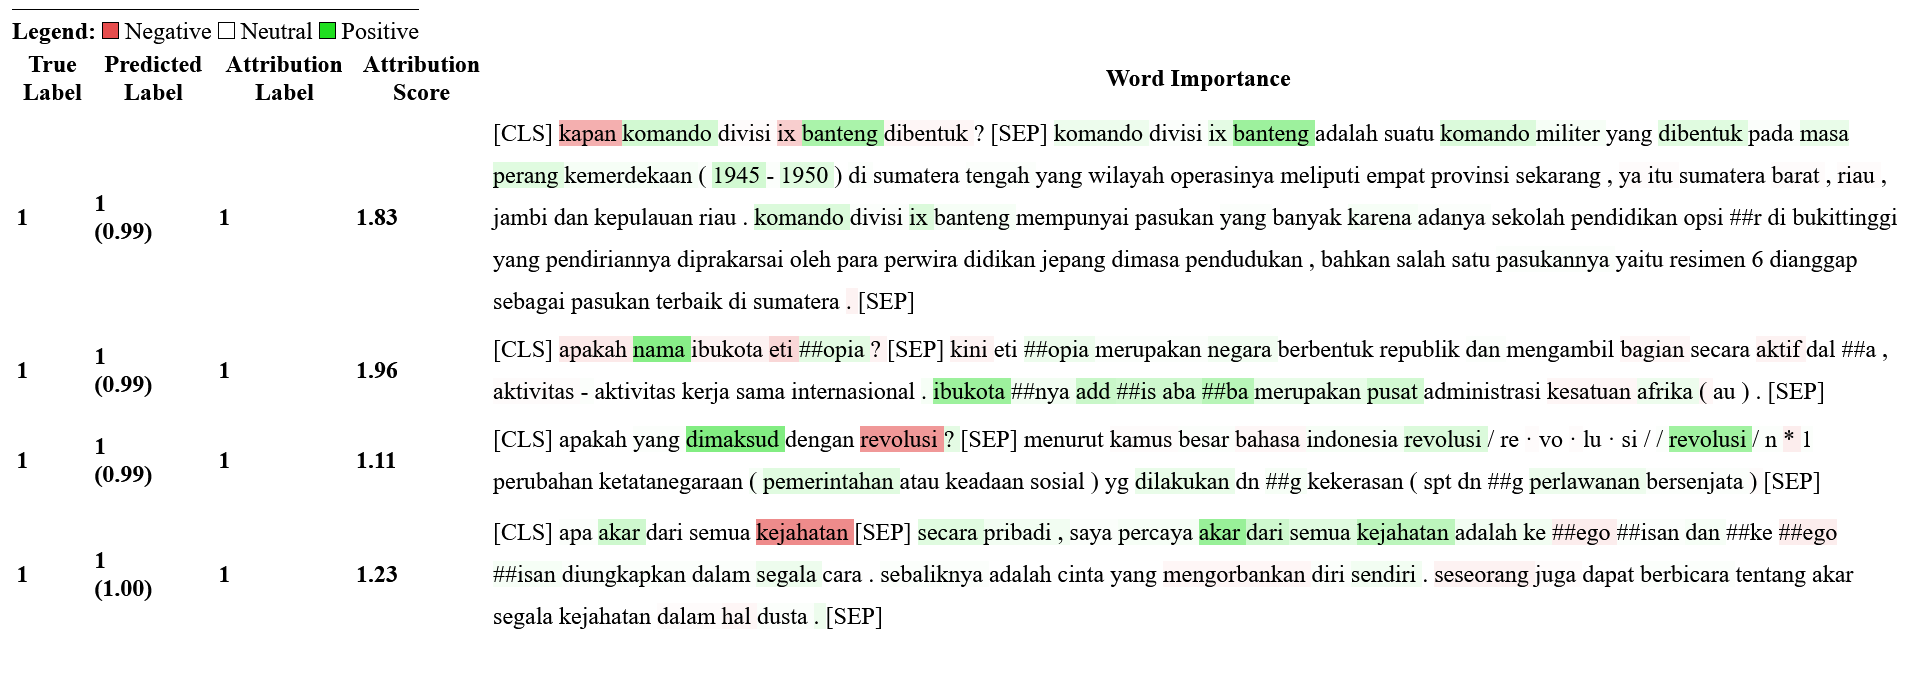
\includegraphics[width=1\textwidth]{assets/pics/IGBERTCAT.png}
    \caption{Interpretasi dari model $\text{BERT}_{CAT}$ dengan \f{integrated gradients}. Kata dengan warna hijau berarti kata tersebut berkontribusi positif terhadap hasil prediksi. Di lain sisi, kata yang berwarna merah berarti kata tersebut berkontribusi negatif terhadap hasil prediksi.}
    \label{fig:InterpretasiBERTCAT}
\end{figure}

Model berasitekturkan $\text{BERT}_{\text{DOT}}$ jauh lebih sulit untuk menginterpretasikannya. Hal yang dapat dilakukan adalah dengan menghitung nilai \f{importance} kata dengan menghitung hasil kali titik representasi vektor dari teks dengan representasi vektor masing-masing kata pada teks tersebut. Dengan hal ini, dapat nilai \f{importance} dari kata dapat diurutkan. \tab~\ref{tab:interpretasibertdot} menunjukkan kueri, teks dan 5 kata penting dari kueri dan teks tersebut.

\begin{table}[!ht]
    \centering
    \caption{Interpretasi dari model $\text{BERT}_{\text{DOT}}$ dengan menghitung hasil kali titik antara vektor teks dengan vektor masing-masing kata pada teks tersebut. Hanya 5 kata dengan nilai \f{importance} tertinggi yang ditunjukkan.}
    \label{tab:interpretasibertdot}
    \begin{tabular}{|p{0.2\textwidth}|p{0.2\linewidth}| p{0.3\linewidth}| p{0.2\linewidth}|}
        \hline
        \textbf{Kueri} & \textbf{ 5 Kata Penting} & \textbf{Teks} & \textbf{ 5 Kata Penting} \\ \hline
        Kapan Petrus Lombardus lahir? & lahir, petrus, kapan, lombardus, ? & Petrus Lombardus mungkin dilahirkan di Novara; atau kemungkinan lainnya adalah di Lumellogno[7] (saat itu sebuah komune pedesaan, sekarang menjadi bagian dari Provinsi Novara, Piemonte), di barat laut Italia, dari suatu keluarga miskin.[8] Kelahirannya diperkirakan antara tahun 1095-1100. & [petrus, dilahirkan, kelahirannya, lombardus, keluarga] \\ 
        \hline
        Dimana Jamie Richard Vardy lahir? & lahir, richard, jamie, ?, dimana & Jamie Richard Vardy (lahir dengan nama Gill; 11 January 1987) adalah pemain sepak bola Inggris yang bermain di klub Premiere League Leicester City dan tim nasional Inggris. Ia bermain sebagai striker, namun juga bisa bermain di sayap & [gill, lahir, richard, tim, sepak] \\
        \hline
    \end{tabular}
\end{table}
